\UseRawInputEncoding
\documentclass[12pt]{article}
\usepackage[utf8]{inputenc}
\usepackage{graphicx}
\usepackage{geometry}
\geometry{letterpaper, margin=2.5cm}
\usepackage{setspace}
\usepackage{lmodern}  % Mejor fuente
\usepackage{titling}  % Para personalizar el título
\usepackage{setspace}

\begin{document}

% Portada manual
\begin{titlepage}
    \centering
    \vspace*{2cm}
    
    {\Large\bfseries Pontificia Universidad Católica de Valparaíso\\[0.2cm]
    Escuela de Ingeniería Eléctrica\\[2cm]}
    
    {\Huge\bfseries Levitación de Bola de Ping Pong\\[0.3cm]
    con Control PID\\[2cm]}
    
    \vfill

    {\large
    Benjamín Malaquías Collao Campos\\[0.2cm]
    Asignatura: Control Automático\\[0.2cm]
    Profesor: Gonzalo Farías C.\\[1.5cm]
    Junio 2025
    }

\end{titlepage}


\newpage


\section*{Introducción}

El siguiente informe describe el desarrollo de un proyecto de control automático con fines pedagógicos, que consiste en mantener una bola de ping-pong levitando a una altura constante mediante un sistema de control PID. El proyecto fue diseñado para ser simple y didáctico, permitiendo comprender el comportamiento de sistemas dinámicos en lazo cerrado, su modelado, análisis y control.

\section{Objetivo}

Diseñar e implementar un sistema de control automático que mantenga una bola de ping pong en suspensión a una altura específica, utilizando un controlador PID.

\section{Armado del proyecto}

El sistema consiste en una aspiradora de mano con batería incorporada, modificada para actuar como generador de flujo de aire vertical. Esta se controla mediante un transistor IRLZ44N, activado por una señal PWM generada por un Arduino UNO. El aire asciende a través de un tubo cilíndrico de acrílico transparente, en cuyo interior se encuentra una bola de ping pong. En la parte inferior del tubo se colocó un cono de papel para centrar el flujo de aire.

El sistema mide la distancia entre la bola y el sensor ultrasónico HC-SR04, ubicado en la parte superior del tubo. Esta señal de retroalimentación se utiliza para ajustar la velocidad del motor de la aspiradora mediante el controlador PID.

\textbf{Materiales principales:}
\begin{itemize}
\item Arduino UNO
\item Sensor ultrasónico HC-SR04
\item Transistor MOSFET IRLZ44N
\item Resistencias de 220 $\Omega$ y 10 k$\Omega$
\item Diodo 1n4001
\item Protoboard, cables dupont
\item Aspiradora de mano con batería (motor)
\item Tubo de acrílico transparente (50 mm de diámetro exterior)
\item Bola de ping pong (38 mm)
\item Cono de cartón piedra (difusor de flujo)
\item Cinta aisladora, silicona caliente, base plástica
\end{itemize}

\subsection{Conexión}

\begin{figure}[h!]
    \centering
    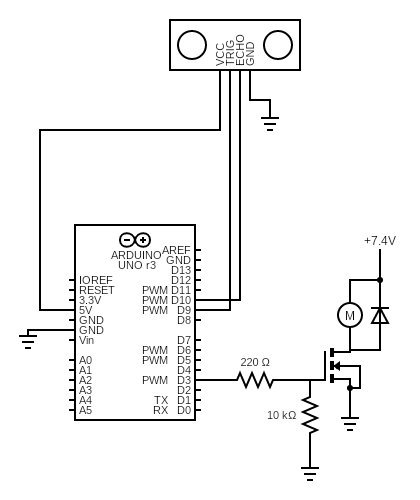
\includegraphics[width=0.5\linewidth]{imagenes/circuit (1).png}
    \caption{Circuito para el proyecto}
\end{figure}

En la Figura 1 se muestra el circuito encargado de controlar el motor de corriente continua utilizado para la levitación de la pelota. El control de velocidad del motor se realiza mediante modulación por ancho de pulso (PWM), generada por un microcontrolador Arduino Uno y aplicada al Gate del MOSFET IRLZ44N. El motor es alimentado directamente por la batería de ion-litio de 7,4V, mientras que el MOSFET permite activar o desactivar el paso de corriente hacia el motor en función de la señal PWM entregada por el Arduino.

Para garantizar el correcto funcionamiento del MOSFET, se ha incorporado una resistencia de 220 ohmios en serie entre el pin digital D3 del Arduino y el Gate del transistor, con el objetivo de limitar la corriente de entrada. Adicionalmente, se incluye una resistencia pull-down de 10 k$\Omega$ entre el Gate y tierra, que asegura que el transistor permanezca apagado cuando no exista señal de control.

El sistema también incorpora un diodo 1N4001 conectado en paralelo al motor, con polaridad inversa. Este componente cumple una función de protección frente a los picos de voltaje generados por la naturaleza inductiva del motor al apagarse, evitando posibles daños en el MOSFET.

Finalmente, el circuito incluye un sensor ultrasónico HC-SR04 conectado a los pines digitales 9 (TRIG) y 10 (ECHO) del Arduino. Este sensor mide la distancia desde el emisor hacia la esfera suspendida, lo que permite retroalimentar el sistema de control PID implementado en el software. Es fundamental que todos los componentes compartan una misma referencia de tierra (GND), para asegurar un comportamiento eléctrico estable y evitar fallos en la comunicación o activación del transistor.
    
\section{Diseño del controlador PID}

Se utilizó un controlador PID debido a su simplicidad, robustez y capacidad de corregir errores sostenidos, adaptarse a variaciones y amortiguar oscilaciones. Los parámetros fueron ajustados mediante prueba y error, observando la respuesta del sistema a perturbaciones y al arranque:

\begin{itemize}
\item $K_p = 6.6$
\item $K_i = 1.9$
\item $K_d = 1.2$
\end{itemize}

Durante las pruebas se documentaron las variaciones de comportamiento en función de los cambios en estos parámetros. El ajuste final logró una buena estabilidad sin oscilaciones graves, manteniendo el setpoint deseado.

\section{Modelo de comportamiento del sistema}

El sistema puede ser modelado como un lazo de control con realimentación negativa. La variable controlada es la distancia entre la bola y el sensor ultrasónico, mientras que la variable manipulada es la señal PWM enviada desde el Arduino hacia el transistor, que regula la velocidad del motor. La planta está compuesta por el motor y la pelota de ping pong suspendida por flujo de aire. Entre las posibles perturbaciones que afectan al sistema se encuentran la turbulencia del flujo de aire y el ingreso accidental de aire por aberturas no deseadas.


\begin{figure}[h!]
    \centering
    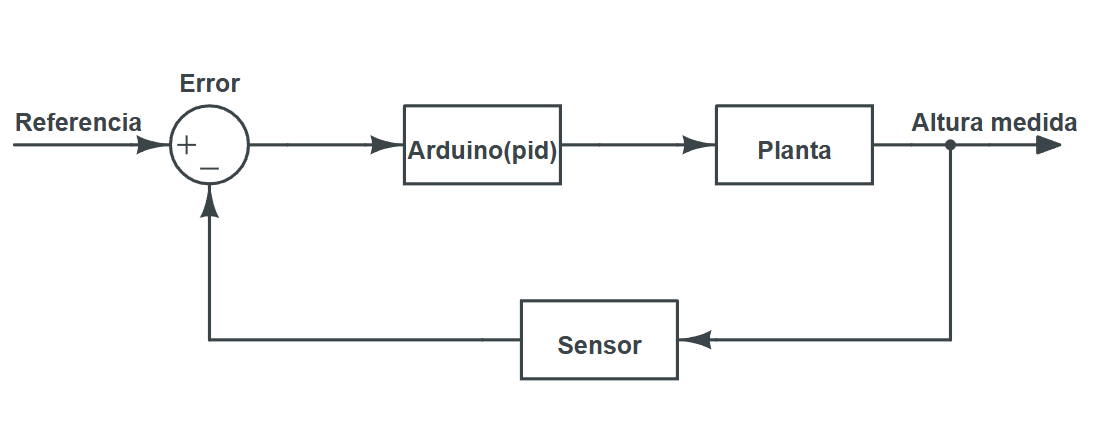
\includegraphics[width=0.9\linewidth]{imagenes/bloques.png}
    \caption{Diagrama de bloques}
\end{figure}

En la Figura 2 se muestra el diagrama de bloques correspondiente. La referencia establece la altura deseada de la bola, la cual se compara con la altura medida por el sensor ultrasónico. El error resultante es procesado por un controlador PID implementado en un microcontrolador Arduino, que ajusta la señal de control hacia la planta. Este sistema permite mantener la bola flotando a la altura deseada mediante una retroalimentación continua.


\section{Resultados y comportamiento del sistema}

El sistema logró estabilizar la bola de ping pong a una altura de aproximadamente 15 cm (setpoint) desde el sensor. El tiempo de estabilización fue de 9 a 10 segundos. Ante perturbaciones (bloqueo parcial o liberación súbita de entradas de aire), el sistema mostró una rápida capacidad de recuperación.

Se observaron oscilaciones leves debido a turbulencias en el flujo de aire y a vibraciones en la estructura del tubo. Estas fueron parcialmente mitigadas con la incorporación de un cono de papel en la base del tubo, que ayudó a centrar el flujo. Además, se utilizó silicona caliente para mantener más estable el tubo en la base. A continuación, se presentan algunas imágenes del proyecto terminado y funcionando.

\begin{figure}[h!]
    \centering
    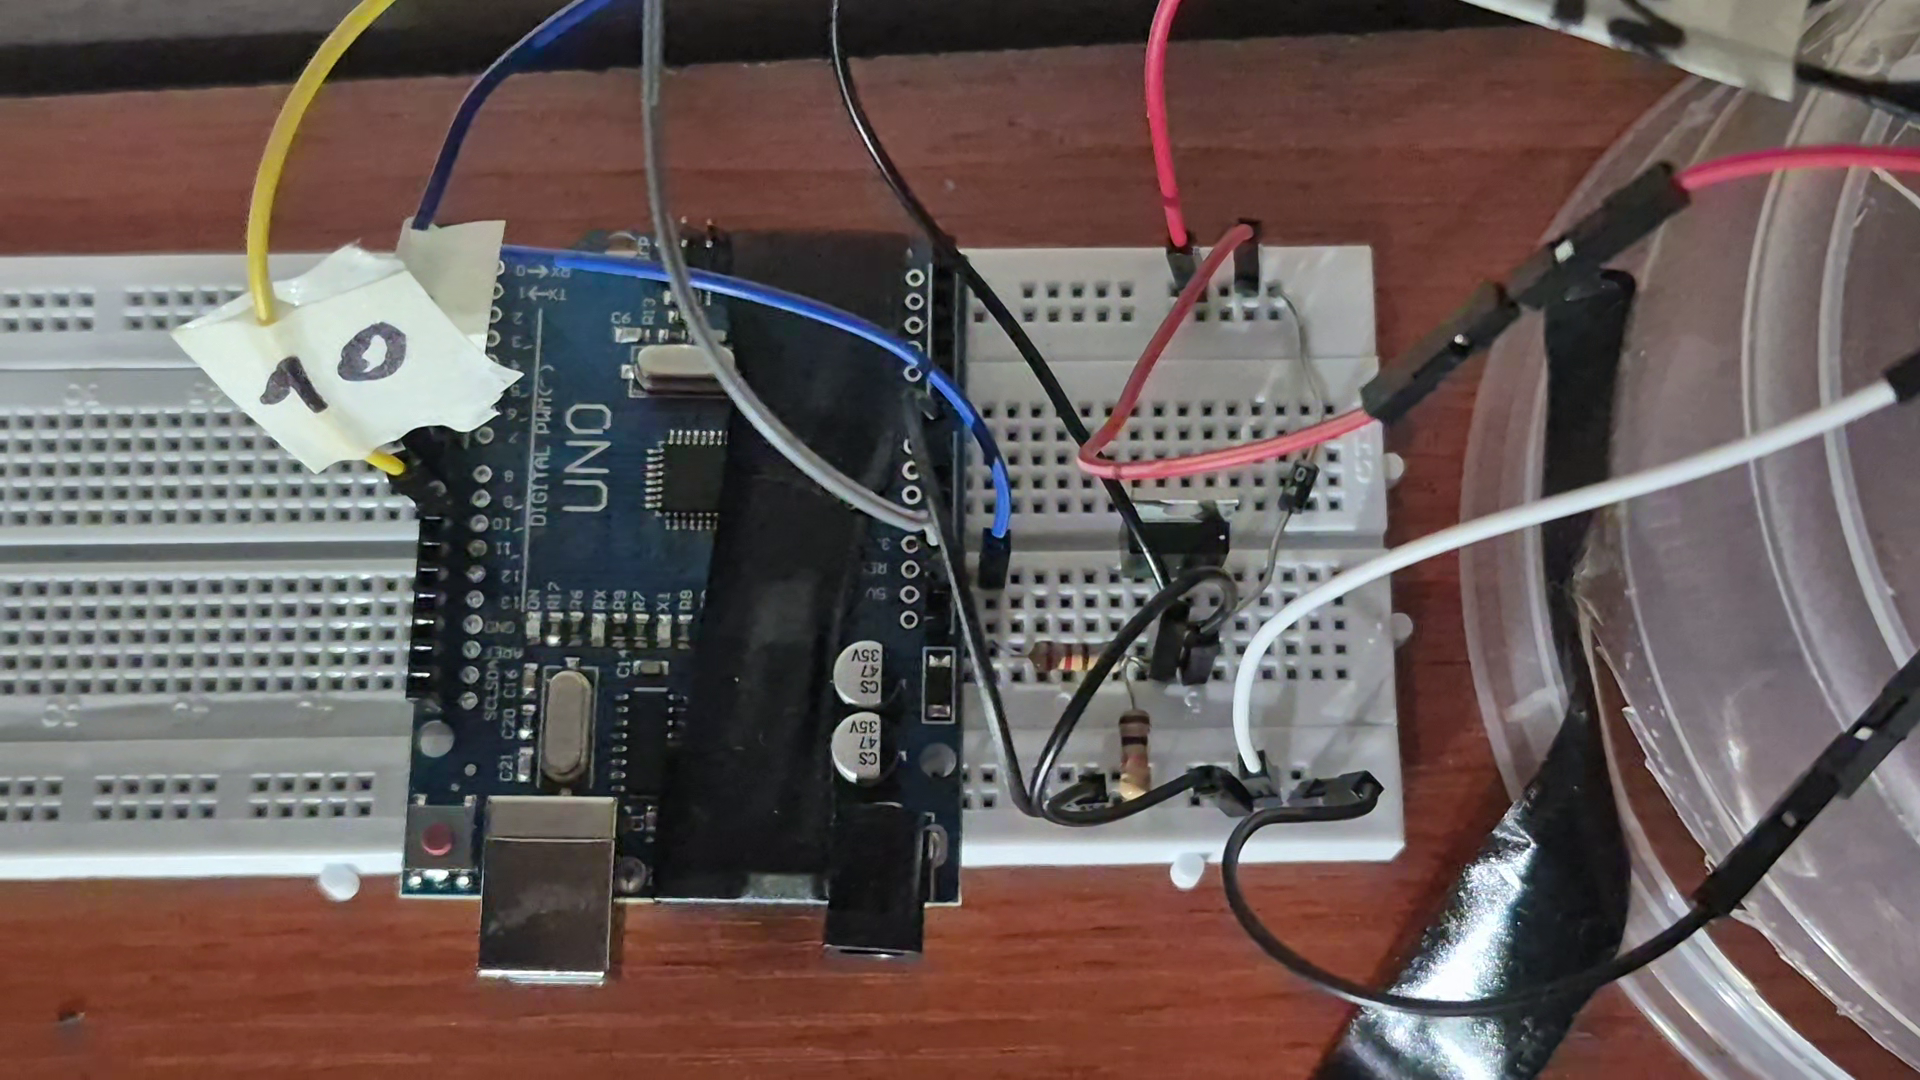
\includegraphics[width=0.7\linewidth]{imagenes/vlcsnap-2025-06-24-01h47m27s949.png}
    \caption{Circuito armado en protoboard}
\end{figure}

\begin{figure}[h!]
    \centering
    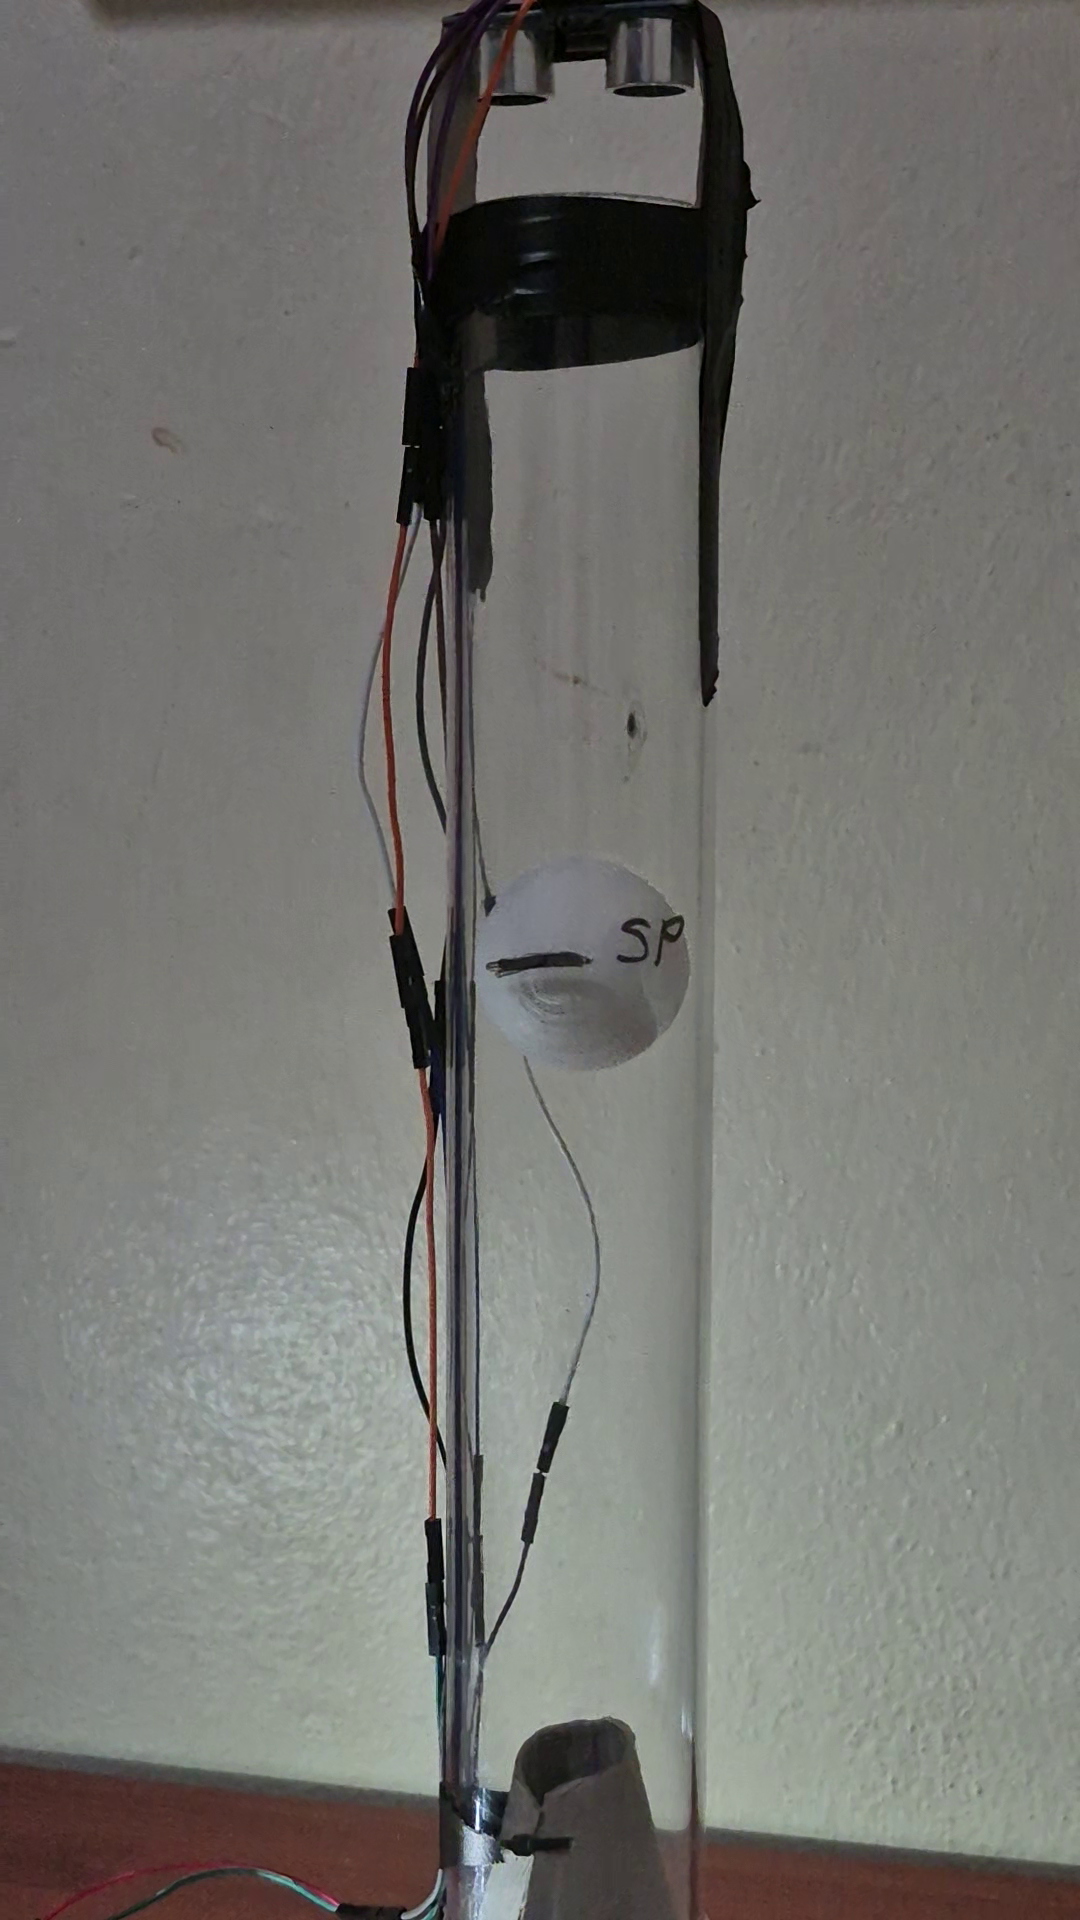
\includegraphics[width=0.4\linewidth]{imagenes/vlcsnap-2025-06-24-01h48m41s111.png}
    \caption{Pelota de ping pong en el setpoint estable}
\end{figure}

\newpage
\section*{Conclusiones}

El proyecto permitió implementar y comprender un sistema de control PID real aplicado a un sistema físico dinámico. Se logró cumplir el objetivo de mantener la bola levitando en una altura específica, con estabilidad y capacidad de respuesta ante perturbaciones. Se evidenció la importancia del diseño físico en el comportamiento del sistema, destacando el impacto de las turbulencias y vibraciones.

Como mejoras futuras se plantea:
\begin{itemize}
\item Incorporar mallas o rejillas para laminar el flujo de aire.
\item Usar un sensor de distancia más preciso y menos sensible a vibraciones.
\item Implementar una etapa de filtrado digital o control adaptativo para compensar errores pequeños.
\end{itemize}

\end{document}


% CODIGO:
%// Pines
const int trigPin = 9;
const int echoPin = 10;
const int motorPin = 3;

// Setpoint deseado
const float setpoint = 15.0;  // distancia en cm

// Variables PID
float input = 0;
float error = 0;
float lastError = 0;
float integral = 0;
float derivative = 0;
float output = 0;

// Constantes PID (ajustadas con prueba y error)
float Kp = 6.6;
float Ki = 1.9;
float Kd = 1.2;

unsigned long lastTime = 0;

void setup() {
  Serial.begin(9600);
  pinMode(trigPin, OUTPUT);
  pinMode(echoPin, INPUT);
  pinMode(motorPin, OUTPUT);
}

void loop() {
  // Medición distancia
  digitalWrite(trigPin, LOW);
  delayMicroseconds(5);
  digitalWrite(trigPin, HIGH);
  delayMicroseconds(10);
  digitalWrite(trigPin, LOW);

  long duration = pulseIn(echoPin, HIGH, 30000);
  input = duration * 0.034 / 2.0;

  // PID simple
  unsigned long now = millis();
  float dt = (now - lastTime) / 1000.0;
  lastTime = now;

  error = input - setpoint;
  integral += error * dt;
  derivative = (error - lastError) / dt;
  output = Kp * error + Ki * integral + Kd * derivative;
  lastError = error;

  // Limitar PWM entre 0 y 255
  output = constrain(output, 0, 255);

  // Aplicar PWM al motor
  analogWrite(motorPin, (int)output);

  // Mostrar en Serial
  Serial.print("Distancia: ");
  Serial.print(input);
  Serial.print(" cm | PWM: ");
  Serial.println(output);

  delay(100);
}